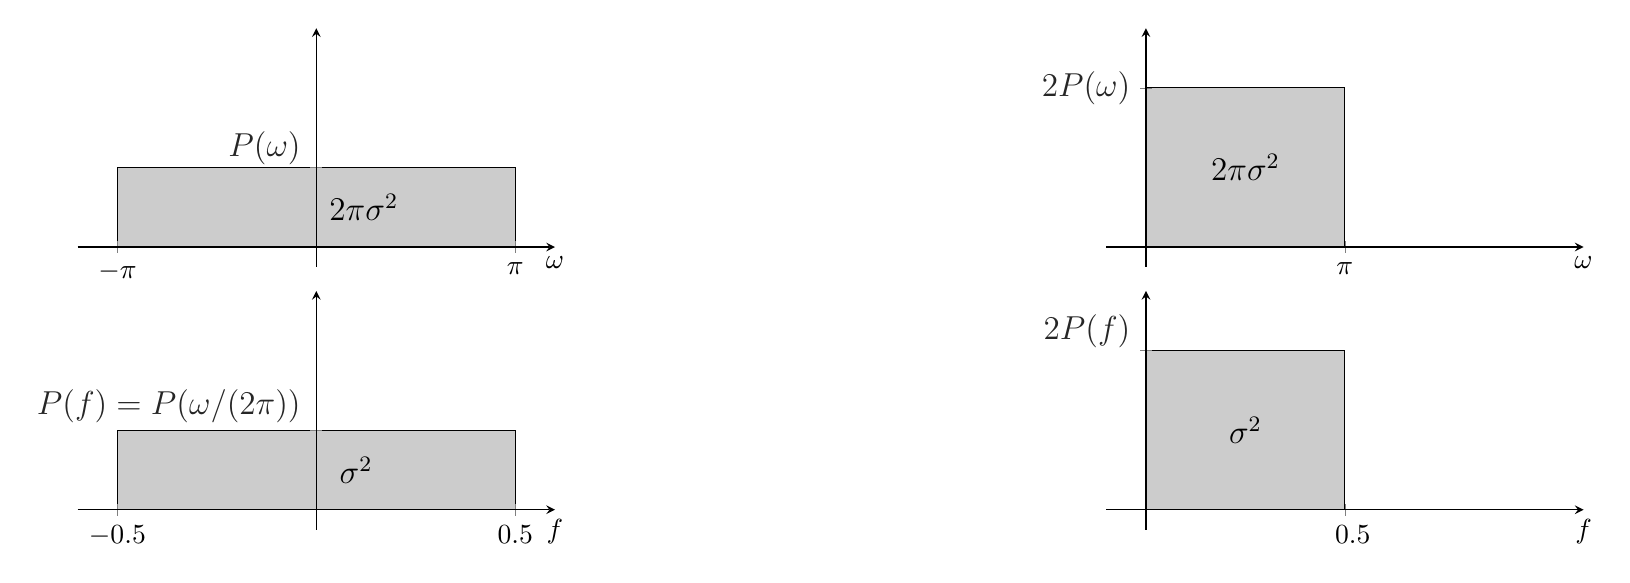
\begin{tikzpicture}
\begin{axis}[
name=plot1,
axis y line=middle, axis x line=middle,
enlargelimits = true, clip=true,
axis on top,
xmin=-3.14, xmax=3.14,
ymin=0, ymax=2.5,
width=0.5\textwidth, height=0.25\textwidth,
axis line style={->,>=stealth},
xlabel={$\omega$},
%ylabel={$P(\omega)$},
scale only axis,
every axis x label/.style={
at={(ticklabel* cs:1)},
anchor=north,
},
every axis y label/.style={
at={(ticklabel* cs:1)},
anchor=south,
},
xtick={-3.14, 0, 3.14}, xticklabels={$-\pi$, $0$, $\pi$},
ytick=1, yticklabels={\large $P(\omega)$},
yticklabel style={yshift=0.25cm},
every outer y axis line/.append style={white!15!black},
every y tick label/.append style={font=\color{white!15!black}},
legend style={draw=white!15!black,fill=white,legend cell align=left}]
\addplot [black, fill=black!20] coordinates {(-3.14, 0) (-3.14, 1) (3.14, 1) (3.14, 0)};
\node at (axis cs: 0.75, 0.5) {\large $2\pi\sigma^2$};
\end{axis}


\begin{axis}[
name=plot2,
at= (plot1.east), anchor=west, xshift=7cm,
axis y line=middle, axis x line=middle,
enlargelimits = true, clip=true,
axis on top,
width=0.5\textwidth, height=0.25\textwidth,
xmin=0, xmax=6.28,
ymin=0, ymax=2.5,
scale only axis,
axis line style={->,>=stealth},
xlabel={$\omega$},
%ylabel={$P(\omega)$},
every axis x label/.style={
	at={(ticklabel* cs:1)},
	anchor=north,
},
every axis y label/.style={
	at={(ticklabel* cs:1)},
	anchor=south,
},
xtick={0, 3.14}, xticklabels={$0$, $\pi$},
ytick=2, yticklabels={\large $2P(\omega)$},
every outer y axis line/.append style={white!15!black},
every y tick label/.append style={font=\color{white!15!black}},
legend style={draw=white!15!black,fill=white,legend cell align=left}]
\addplot [black, fill=black!20] coordinates {(0, 0) (0, 2) (3.14, 2) (3.14, 0)};
\node at (axis cs: pi/2, 1) {\large $2\pi\sigma^2$};
\end{axis}

\begin{axis}[
name=plot1a,
at=(plot1.below south east), anchor=above north east,
axis y line=middle, axis x line=bottom,
axis on top,
enlargelimits = true, clip=true,
width=0.5\textwidth, height=0.25\textwidth,
scale only axis,
axis line style={->,>=stealth},
axis y line=middle, axis x line=middle,
enlargelimits = true, clip=true,
xmin=-0.5, xmax=0.5,
ymin=0, ymax=2.5,
axis line style={->,>=stealth},
xlabel={$f$},
%ylabel={$P(f)$},
every axis x label/.style={
	at={(ticklabel* cs:1)},
	anchor=north,
},
every axis y label/.style={
	at={(ticklabel* cs:1)},
	anchor=south,
},
xtick={-0.5, 0, 0.5},
ytick=1, yticklabels={\large $P(f) = P(\omega/(2\pi))$},
yticklabel style={yshift=0.3cm},
every outer y axis line/.append style={white!15!black},
every y tick label/.append style={font=\color{white!15!black}},
legend style={draw=white!15!black,fill=white,legend cell align=left}]
\addplot [black, fill=black!20] coordinates {(-0.5, 0) (-0.5, 1) (0.5, 1) (0.5, 0)};
\node at (axis cs: 0.1, 0.5) {\large $\sigma^2$};
\end{axis}

\begin{axis}[
name=plot2a,
at= (plot1a.east), anchor=west, xshift=7cm,
axis y line=middle, axis x line=middle,
enlargelimits = true, clip=true,
axis on top,
width=0.5\textwidth, height=0.25\textwidth,
scale only axis,
xmin=0, xmax=1,
ymin=0, ymax=2.5,
axis line style={->,>=stealth},
xlabel={$f$},
every axis x label/.style={
	at={(ticklabel* cs:1)},
	anchor=north,
},
every axis y label/.style={
	at={(ticklabel* cs:1)},
	anchor=south,
},
xtick={-0.5, 0, 0.5},
ytick=\empty,
xticklabel style={xshift=0.1cm},
ytick=2, yticklabels={\large $2P(f)$},
yticklabel style={yshift=0.25cm},
every outer y axis line/.append style={white!15!black},
every y tick label/.append style={font=\color{white!15!black}},
legend style={draw=white!15!black,fill=white,legend cell align=left}]
\addplot [black, fill=black!20] coordinates {(0, 0) (0, 2) (0.5, 2) (0.5, 0)};
\node at (axis cs: 0.25, 1) {\large $\sigma^2$};
\end{axis}
\end{tikzpicture}